\documentclass[a4paper,oneside,12pt]{article}

\usepackage{standalone}

\usepackage{vhistory}
\usepackage{setspace}

\usepackage{url}
\usepackage[utf8]{inputenc} 
\usepackage[english,danish]{babel} 
\usepackage{lmodern} % Modern LaTeX font
\renewcommand{\danishhyphenmins}{22} 
\usepackage[T1]{fontenc}
\usepackage{amsmath,amssymb,bm,mathtools}
\usepackage{gensymb}
\usepackage[load-configurations=version-1]{siunitx}
\usepackage{graphicx}
\usepackage{svg}
\usepackage{float}
\usepackage{setspace}
\usepackage[font=footnotesize]{caption}
\usepackage{fancyhdr}

\usepackage[style=ieee]{biblatex}
\addbibresource{biblio.bib}

\pagestyle{fancy}


\begin{document}
\begin{titlepage}
\centering
\vfill
{\LARGE Rapport}\\
\vfill
{\bfseries\large
	Bachelorprojektet: \\
	Real-time eye-tracking\\
	Projektnummer: 15017\\
}
\vfill

\includegraphics{ASE_logo.png}
\vfill
{\bfseries\large
	25/05/2015\\
	Studerende: Søren Vøgg Krabbe Lyster (SVL) 10920,\\
	Martin Degn Kristensen (MDK) 10441\\ 
	Studieretning: Elektro \\
	Vejleder: Preben Kidmose \\
	\vfill	
	\rule{6cm}{1pt}
}




\end{titlepage}
\lhead{
\includegraphics[scale=0.2]{ASE_logo.png}}
\chead{Real-time eye-tracking}
\rhead{\scriptsize 25/05/15 \\
S. V. K. Lyster, M. D. Kristensen}
\tableofcontents
\documentclass[rapport.tex]{subfiles}

\begin{document}

\section{Prolog}
	\subsection{Indledning}
	Denne rapport er udarbejdet som afslutningen på 7. semester bachelorprojekt i Elektro på Ingeniørhøjskolen Aarhus Universitet. Projektet er udbudt af Preben Kidmose ved Ingeniørhøjskolen Aarhus Universitet. I et EEG-system (Elektroencephalografi) ønskes der detekteret hvor på en skærm en testpersons øjne er fokuseret (gaze vector). Ved at observere dette kan EEG-målinger sammenholdes med visuel stimuli. Dette projekt omhandler implementeringen af en software-løsning der tillader realtids-målinger af en testpersons gaze vector. Software-løsningen skal fungere som et application programming interface (API) for en eye-tracking algoritme, således at projektudbyder m.fl. kan implementere egen algoritme, uden at skulle kende til resten af softwarens struktur.  Forud for projektet er der givet en hardware-løsning der designes ud fra. For at teste og benytte API'en er der også implementeret en udgave af eye-tracking-algoritmen kendt som Starburst-algoritmen. To eksemplarer af Starburst-algoritmen er givet på forhånd: Daniel Siboska's MATLAB-implementering og OpenEyes C-implementering. 
	
	\subsection{Krav til bachelorprojekt}
	Aarhus Universitets kursuskatalog beskriver følgende krav til bachelorprojekt på Ingeniørhøjskolen:\\
	
	
\textit{	Ingeniøruddannelsen afsluttes med et bachelorprojekt, som skal dokumentere den studerendes evne til at anvende ingeniørmæssige teorier og metoder inden for et fagligt afgrænset emne. }\\

	
\textit{	Når kurset er afsluttet, forventes den studerende at kunne: 
}	
	\begin{itemize}
		\item\textit{ Anvende videnskabelige forskningsresultater og indsamlet teknisk viden til løsning af tekniske problemstillinger}
		\item \textit{Udvikle nye løsninger}
		\item \textit{Tilegne sig og vurdere ny viden inden for relevante ingeniørmæssige områder}
		\item \textit{Udføre ingeniørmæssige rutinearbejde indenfor fagområdet}
		\item \textit{Kommunikere resultater af et projekt skriftligt til fagfolk såvel som kunder}
		\item \textit{Præsentere resultater af et projekt mundtligt og ved hjælp af forskellige audiovisuelle kommunikationsværktøjer}
		\item \textit{Integrere sociale, økonomiske, miljømæssige og arbejdsmiljømæssige konsekvenser i en løsningsmodel.}
	\end{itemize}
	
	\subsection{Ordforklaring}
		\item \textbf{Gaze Vector}: Dette term bruges om den vektor som beskriver hvor en person ser hen. Denne vektor er et af de resultater der ønskes fra eye-tracking systemet.
		\item \textbf{Session}: Dette term bliver brugt om en real-time eye-tracking måling foretaget af i programmet. Sessionen beskriver det enkelte målingsforløb fra start til slut. Til hver session vil der være tilknyttet separate præference- og logfiler. 
		\item \textbf{Data-fil}: Dette er den fil der vil blive tilknyttet til hver session. Filen vil forventes at indeholde al relevant data i forbindelse med real-time eye-tracking måling. Filen vil blive kreeret af programmet og vil være tilgængelig til brugeren. 
		\item \textbf{Testperson}: Det er denne person der foretages real-time eye-tracking på. Personen er sammen med brugeren en del af kalibreringsrutinen. Denne person ses ikke som aktør i systemet. 
		\item \textbf{Trigger}: For at kunne holde en synkronisering imellem real-time eye-tracking softwaren og andre målinger (EEG), er der givet et trigger-signal. Dette signal består af en ændring af lys-intensitet. 
		\item \textbf{API (Application programming interface)}: Betegnelsen der bruges for den softwaregrænseflade der ønskes implementeret til afvikling af eye-tracking-algoritmer. 
		\item \textbf{Timestamp}: Det klokkeslet i timer, minutter, sekunder og millisekunder der ønskes skrevet i logfilen. 
	\subsection{Projektformulering}
	Fra projektoplægget er føljende beskrivelse givet:\\
	\\
\textit{	Eye-tracking is widely used in different research areas as for example in psychology, in analysis of man-computer interactions, and in behavioural studies. Eye-tracking is also used in computer gaming. At ASE eye-tracking is used for research both in the biomedical lab and in the vision lab. The system as it is now is based on off-line Matlab processing of camera data. The purpose of this project is to design and implement a software system for real-time acquisition of the eye-movements. The basic principle of the eye-tracking system is based on reflection from two IR-LED’s from the eyes. By identifying the reflections, and doing some geometrical computations, it is possible to determine the users gaze vector. 
	The project will build on an existing hardware setup comprising a camera, IR-sources and a computer screen. The primary objective of the project is to design and build a flexible software system that can process the camera data in real-time, and output the gaze vector. The image processing will build on an existing Matlab implementation. The system must be designed such that there is a flexible interface to the image processing part in order to facilitate new image processing algorithms to be tested in the system. For students with particular interest in image processing, a secondary objective could be to further develop on the image processing algorithms.} 
	\\
	
	\subsection{OpenEyes og Siboska}
	Den implementerede udgave af Starburst-algoritmen har taget udgangspunkt i de to løsninger givet af Daniel Siboska \cite{Siboska} og OpenEyes open source eye-tracking kode \cite{openEyes}.  
	
		
\end{document}
\documentclass[rapport.tex]{subfiles}

\begin{document}
\section{Metode}
	\subsection{Metoder}
	Til dette projekt er der blevet benyttet V-modellen som udviklingmetode \cite{Vmodel}, og UML (Unified Modelling Language) \cite{UML} til design af softwarearkitekturen . V-modellen tilbyder en overskuelig tilgang til softwareudvikling i et projekt hvor en række krav er fastsat som udgangspunkt for udviklingen. Ved hjælp af UML er de forskellige krav omskrevet til use cases, og derfra er der udviklet design-diagrammer for softwarearkitekturen. 
	V-modellen følger i dette projekt følgende stadier fra analyse til implementering:
	\begin{itemize}
		\item Opstilling af krav
		\subitem Ud fra projektoplægget og samtaler med projektudbyderen kan der formuleres en række konkrete krav til systemet. Disse krav kan deles op i funktionelle og ikke funktionelle krav. De funktionelle krav er direkte tilknyttet systems funktionalitet, hvor de ikke funktionelle krav i dette projekt omhandler ting som for eksempel præcision og opdateringshastighed. Dette stadie ender ud i færdiggørelsen af en kravspecifikation. 
		\item Analyse
		\subitem
		\item Design
		\subitem Ud fra de opstillede use cases kan der udvikles designdiagrammer til systemet. Disse diagrammer er udarbejdet udfra UML, og indeholder derfor en tydelig overgang fra use case. Sekvensdiagrammer er designet for hver use case, og resulterer i en række ønskede klasser. Klasserne defineres mere specifikt i klassediagrammer. Programmets flow-struktur designes således at der er en fornuftig kommunikationsvej fra det grafiske bruger-interface, til selve eye-tracking algoritmen. Et udkast til det grafiske bruger-interface bliver skitseret således at al funktionalitet fra de opstillede krav kan opfyldes. Et flow-diagram for Starburst algoritmen designes. Dette stadie ender ud i et softwarearkitektur-dokument. 
		\item Implementering
		\subitem ORDORDORD
	\end{itemize}	
	Efter implementering af koden følger modellen en række test-stadier:
	\begin{itemize}
		\item Deltest
		\subitem Deltest tester den individuelle klasses funktionalitet op imod softwarearkitekturen. Herved kan eventuelle fejl og mangler fanges tidligt. 
		\item Integrationstest
		\subitem Her testes de forskellige klassers interaktion med hinanden. Der undersøges om klasserne sender de rigtige data, og om der bliver gjort de rigtige funktionskald. 
		\item Accepttest
		\subitem Accepttesten er den endelige test af systemet. Her undersøges om systemet i sin helhed lever op til de forskellige krav formuleret i kravspecifikationen. \\
		
	\end{itemize}
	
	
	V-modellens fleksibilitet tillader at man ved hvert teststadie kan gå tilbage og tilpasse analyse, design og implementering. 
	V-modellen giver derfor mulighed for at opstille en række krav, omskrive dem til softwarearkitektur, implementere arkitekturen, foretage tests på den implementerede kode, og derefter gå tilbage rette hvad der kunne være nødvendigt. 
	I et projekt af denne størrelse, hvor det forventes at der skal tilegnes ny viden, giver denne model derfor god mulighed for tidligt at støde på eventuelle problemer ved implementeringen, og derefter søge ny viden der kan benyttes til at opnå de opstillede krav. 
	
	\subsection{Planlægning}
	Bacheloropgaven er sat til 20 ECTS point, hvilket ifølge Aarhus Universitet svarer til 560 timer. Bachelorprojektets forløb strækker sig fra januar til slut maj, og er anslået til at vare 20 uger. Derudover har der været et forprojekt i december 2014. Der er derfor bestemt et gennemsnitligt arbejdspres på 30 timer om ugen for hele forløbet. I samarbejde med vejleder er der aftalt en times møde hver mandag. Desuden har det været bestræbt at mødes i projektgruppen hver hverdag, med forbehold for sygdom og således. Internt i projektgruppen har det været aftalt af føre personlig logbog, hvori overvejelser og noter kunne føres. \\
	\\
	Tidsplan for projektet (se figur \ref{fig:Tidsplan}) er blevet udført i løbet af forprojektet med henblik på projektstruktur som angivet af v-modellen. Denne tidsplan er blevet revideret og opdateret til vejledermødet hver mandag. 
	
	\begin{figure}
	\centering
	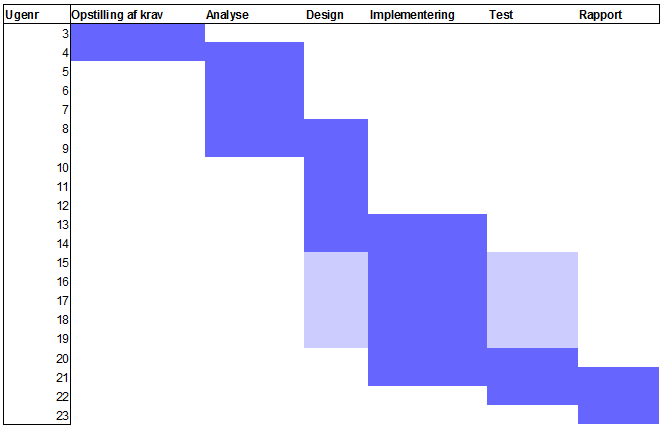
\includegraphics[width=1\linewidth]{Tidsplan}
	\caption{Tidsplan for projektet. Mørkeblå farve viser den konkrete tidsplan. lyseblå farve viser perioder hvor det forventedes at de forskellige stadier ville overlappe hinanden.}
	\label{fig:Tidsplan}
	\end{figure}
	
	\subsection{Diskussion}
	
		
\end{document}
\documentclass[rapport.tex]{subfiles}

\begin{document}
\section{Værktøjer}
	\subsection{Udviklingsmiljø}
	Eye-tracking programmet er blevet udviklet delvist i Pythons IDE Idle, og delvist i Microsofts Visual Studio. Al kode er versionsstyret ved hjælp af versionsstyringssystemet Git. Arbejde med UML, samt design af diverse diagrammer og figurer, er udført i Microsofts Visio. 
	\subsection{OpenCV}
	OpenCV er et programbibliotek frit tilgængeligt under BSD licensen. Programbiblioteket tilbyder optimerede funktioner designet med henblik på hurtige udregninger med fokus på realtids-programmering. Desuden giver OpenCV en række funktioner for kommunikation med video-hardware, samt behandling af videofiler. OpenCV's funktioner er implementeret i kodesproget C++, men understøtter implementering igennem både Python, Java og Matlab, og kører på Windows, Linux, OS X, Android m.m. \cite{opencv}.
	\subsection{Python}
	Python er et høj-niveau kodesprog der understøtter objekt-orienteret programmering, miksede høj-niveau datatyper, automatisk memory management, og et ekstensivt programbibliotek. 
	Python understøtter derfor hurtig implementering i forhold til både Java og C++. Desuden understøtter Python også wrapping med C/C++. Dette er basis for arbejde med OpenCV.  
	\subsubsection{Python vs. Java og C++} 
	
	Fordele \cite{PythonComp}: \begin{itemize}
		\item 3-5 gange kortere end Java og 5-10 gange kortere end C++. 
		\item Automatisk garbage collector. Ingen fokus på frigørelse af resourcer. 
		\item Miksede høj-niveau datatyper.
	\end{itemize}
	Ulemper: \begin{itemize}
		\item Langsommere end bade Java og C++, da datatyper skal ikke nødvendigvis er defineret før runtime. 
	\end{itemize}
	
	\subsubsection{Relevante programbiblioteker}
	Nogle af Python's benyttede programbiblioteker har haft stor indflydelse på projektet, og er derfor relevante at nævne: \\\\	
	\textbf{Numpy} er et højt optimeret programbibliotek til arbjede med numeriske operationer og tilbyder derfor en god understøttelse af array- og matrice-matematik, samt en ekstensiv række høj-niveau matematiske funktioner \cite{Numpy}. Numpy er derfor anvendt af OpenCV i Python. \\\\
	\textbf{Tkinter} er en Python-binding til GUI-værktøjet Tk. Dette interface giver mulighed for en nem implementering af det grafiske bruger-interface, og er frit tilgængeligt under en Python-licens \cite{Tkinter}.

	\subsection{Diskussion}
	Det valgte udviklingsmiljø har givet et sæt stærke værktøjer til design, implementering, debugging og profiling. Versionsstyring har været de naturlige valg når det kommer til programmering. 
	Brugen af Numpy har lagt grund for en nem omskrivning af Siboskas MATLAB-kode, da de fleste matematiske funktioner også findes i Numpy. 
		
\end{document}
\documentclass[rapport.tex]{subfiles}

\begin{document}
\section{Kravspecifikation}

	\subsection{Problemstillinger}
	Der ønskes udviklet et system som kan indsamle videodata fra et kamera og derefter anvende dataen til
	at bestemme hvor en forsøgsperson kigger hen på en specifik skærm. Systemet skal derudover videregive
	denne information til brugeren via koordinater samt en graf der repræsenterer den skærm forsøgspersonen
	ser på.
	\\
	\indent
	Før dataopsamling skal en indledende kalibrering af systemet gennemføres. Dette gøres ved at et gitter med
	specifikke punkter indlæses på forsøgspersonsskærmen. Derefter bedes forsøgspersonen fiksere på specifikke punkter
	på skærmen, og sammenhængen imellem de målte punkter og de kendte punkter kan anvendes til at finde en
	homografisk mapning. Efter denne kalibrering kan systemet anvendes.
	\\
	\indent
	Systemet udvikles med henblik på en standard anvendelsesmåde, med mulighed for brugerdefinerede anvendelsesmåder. 
	Standardanvendelsen omhandler at vælge en sti og et filnavn, hvorefter dataopsamling umiddelbart begynder.
	Under dataopsamlingen vil gazevectoren løbende blive præsenteret for brugeren på brugerskærmen. Når brugeren er 
	færdig kan opsamlingen stoppes, og dataopsamlingen gemmes i den tidligere valgte fil. Bemærk at den algoritme
	der anvendes til behandling af data her er forudbestemt.
	\\
	(Hvis brugeren ønsker at bruge en anden algoritme kan denne indlæses. Den kan også indskrives direkte i
	GUI'en, og derefter gemmes. Formålet med dette er at kunne indrette systemet efter specifikke behov, og
	hurtigt indhente de opsætninger til fremtidig brug. Eventuelt kan andre variabler indtastes ved systemstart) 
	\\
	\indent
	I de følgende afsnit fremgår det hvorledes det udviklede system indgår i det samlede system.
	
	
	\subsection{Funktionelle krav}
	Følgende funktionelle krav for systemet er blevet stillet: \\
	\begin{enumerate}
		\item 
		\textbf{Real-time eye-tracking}: Systemet skal kunne foretage real-time eye-tracking.
		\item 
		\textbf{Kalibrering}: Før måling skal programmet kunne kalibreres.
		\item
		\textbf{Output}: Resultater af måling skal ende i en log-fil tilgængelig til brugeren.
		\item
		\textbf{Brugertilgang}: Ved hjælp af use case teknikken vil en yderlige række krav blive stillet. Disse vil lægge grundlag for bruger-program-interaktioner. Use-case-kravene er opstillet i afsnit \ref{usec}.  
	\end{enumerate}
	
	\subsection{Kalibrering}
	Kalibrering: Specifikke ukendte variabler skal kunne kalibreres ved hjælp af interpolation. Herved skal programmet kunne tilpasses testpersonens fysiske forhold til kameraet. 
	\begin{figure}[h]
		\centering
		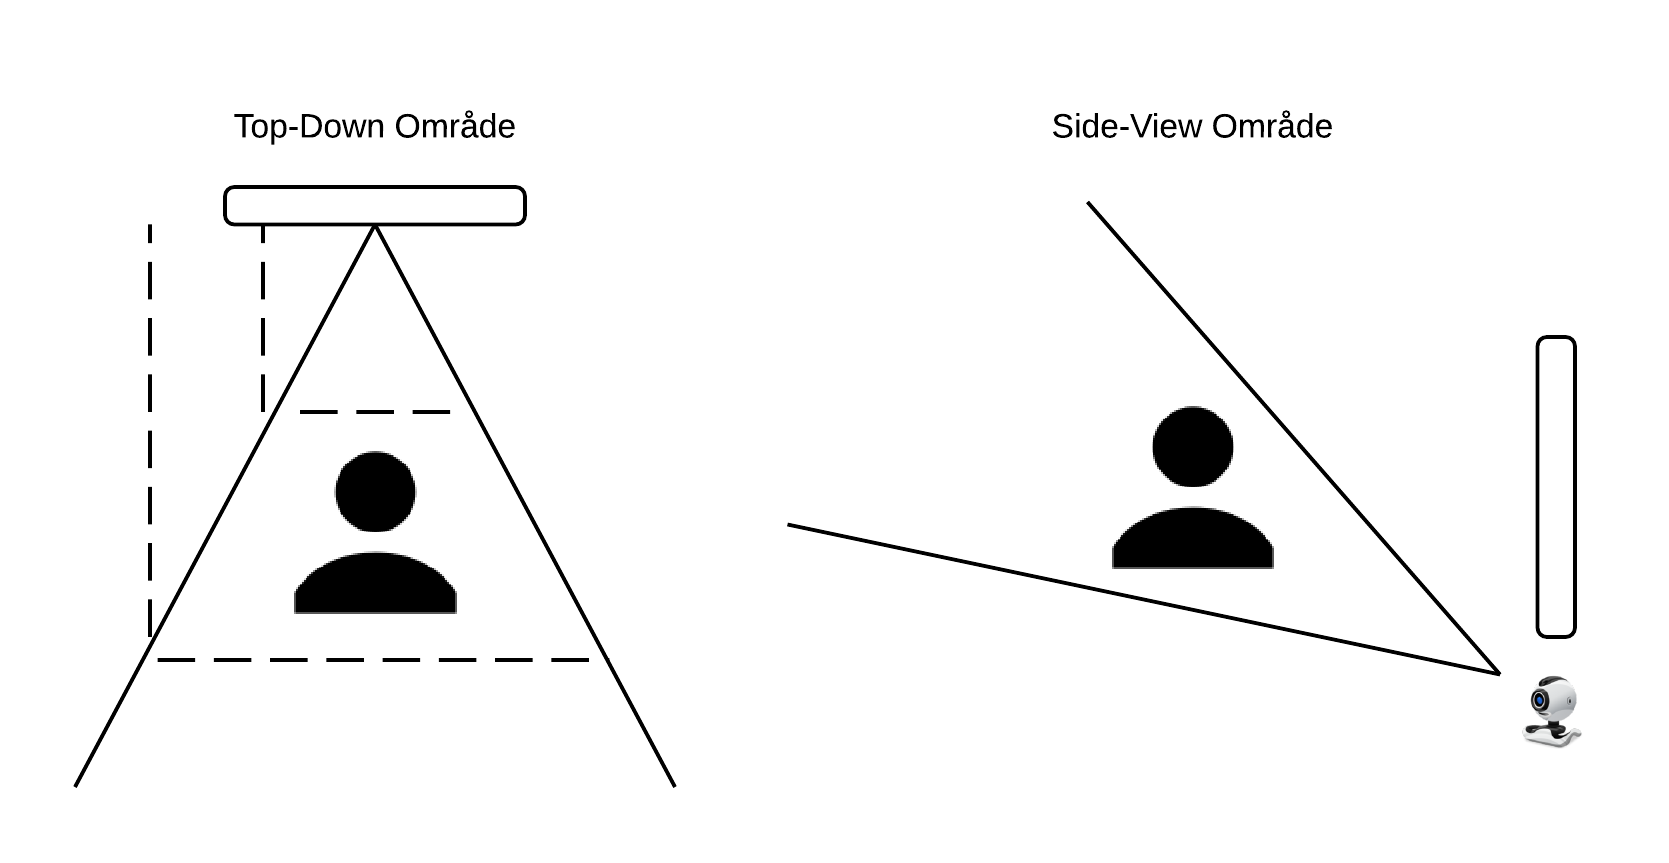
\includegraphics[width=0.7\linewidth]{../Kamera-testperson}
		\caption{Kameraets position i forhold til testperson}
		\label{fig:Camposition}
	\end{figure}
	
	
	Derudover skal programmet kunne kalibreres således at der kan findes tærskler (threshold-values) for trigger-niveauet: En værdi når trigger-niveauet går højt, og en værdi når trigger-niveauet går lavt.
	
	\begin{figure}[H]
		\centering
		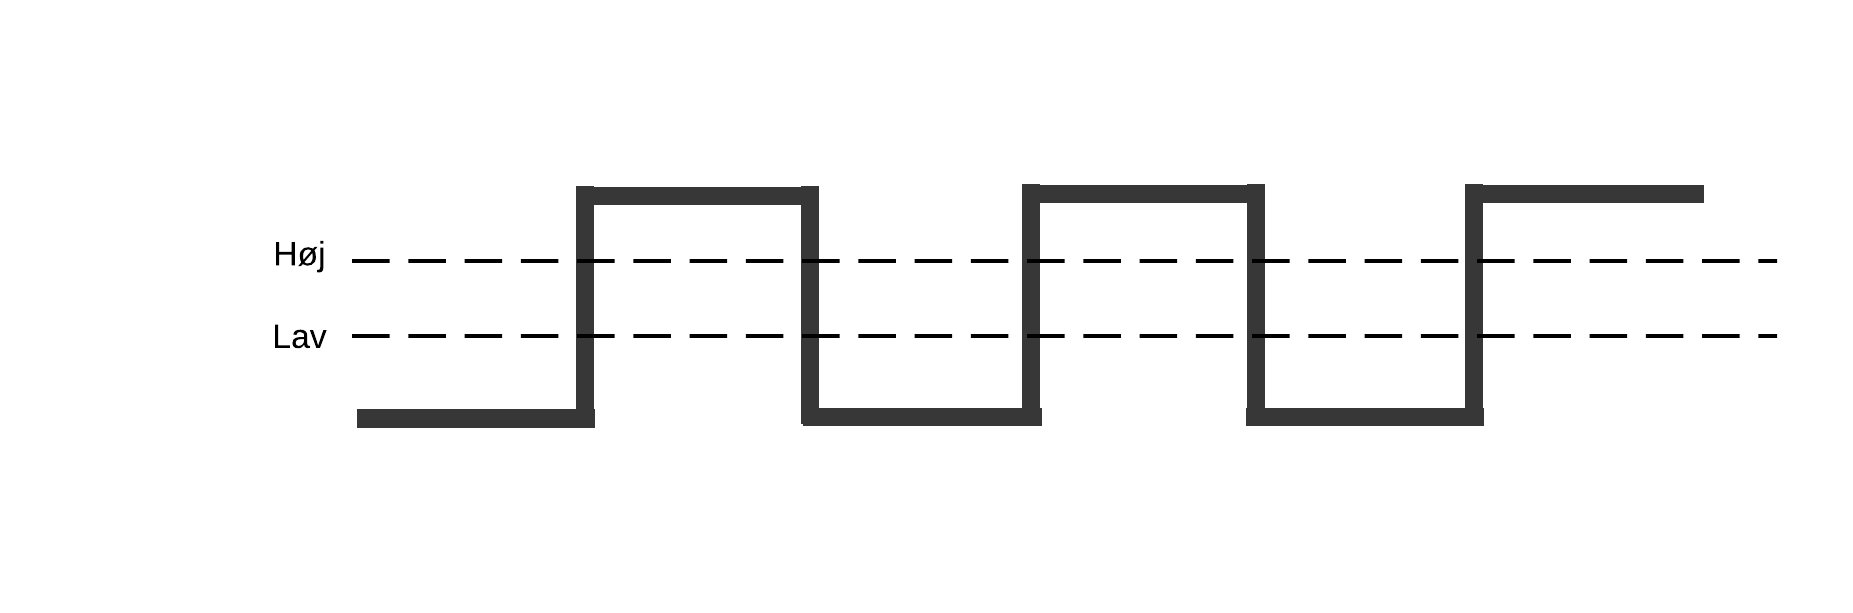
\includegraphics[width=0.7\linewidth]{../Trigger-threshold}
		\caption{Eksempel på tærskelværdier for trigger-signalet}
		\label{fig:Trigger-threshold}
	\end{figure}
	
	
	
	\subsection{Output}
	For hver igangsat session skal programmet generere en log-fil med følgende data:
	\indent \begin{itemize}
		
		\item 	Kommasepareret målingsdata med følgende format: \\
		\textit{X-koordinat, Y-koordinat, Samplenummer, Trigger-niveau (0 for lav, 1 for høj)} 
	\end{itemize}
	
	\subsection{Use-cases}	
	\label{usec}
	\begin{enumerate}
		\item Opret session: \\Opretter en session i en fil-sti med nødvendige data-filer. 
		\item Kalibrering: \\Initierer en række kalibreringer før brug. 
		\item Start måling: \\Igangsætter måling.
		\item Stop måling: \\Afslutter måling.
		\item Gem indstillinger: \\Gemmer en fil med brugerens nuværende indstillinger.
		\item Indlæs indstillinger: \\Indlæser indstillinger fra gemt fil.
		\item Indlæs rå data: \\Indlæser rå data fra tidligere session. 
	\end{enumerate}
	\subsection{Ikke funktionelle krav}
	Real-time eye-tracking systemet skal leve op til en række ikke funktionelle krav. Disse krav skal garantere et robust system, der med en hvis præcision skal kunne levere de ønskede data.\\
	\begin{itemize}
		\item 
		\textbf{Fejlmargin}: Systemet skal kunne angive XY-koordinater for øjets fokuspunkt. Disse koordinater må have en afvigelse på <2\degree \cite{FairchildInSiboska}.
		\item 
		\textbf{Real-time}: Systemet skal kunne angive XY-koordinater med en frekvens bestemt af kameraets frame-rate. 
		\item
		\textbf{Kamera}: Skal kunne levere video-data real-time til en computer. Systemet bliver udviklet til kamera af typen Basler
		ACA640-100gc GigE med opløsningen 658 x 492 pixels og maksimum framerate på 100Hz.
		\item Følgende krav er ikke krav til systemet, men krav til testpersonens fysiske forhold til kameraet. Dette er relevant når der foretages eye-tracking. \\
		\textbf{Afstand og skærm}: Systemet bliver udviklet med en afstand fra kamera til testperson på 60m. 
		På samme afstand fra testpersonen er der placeret en skærm. Denne skærm har størrelsen 26 tommer.
	\end{itemize}
	
	Typen af kamera og afstand til testperson kommer fra tidligere forsøg \cite{Siboska}.
	\subsection{Performance-evaluering}
	\subsection{Diskussion}
	
		
\end{document}
\documentclass[rapport.tex]{subfiles}

\begin{document}
\section{Analyse}
	\subsection{Indledning}
	Formålet med analysedelen af projektet var at få en indledende indsigt i emnet. Det indebar at få skabt et overblik over hvad der skullealaves, hvorfor det skulleal les, og hvilke krav der er til de ting som skulle lavesal lavdover er det også vigtigt at nævne at det der bliver diskuteret overvejende er koncepter eller teori, med enkelte eksempler som kan øge forståelsen for meningen. Konkret design og implementering vil blive gennemgået senere, i design og implementeringsdelene af rapporten.
	\subsection{Systemoversigt}
	
	Blokdiagram: Userskærm, testskærm, IR-LED, kamera.
	Blokdiagram2: Overordnet blokdiagram over software. (Figur 2, geometric approach to eyetracking)
	
	Billede af opstilling.
	
	
	
	
	Dette er opstillingen som projektet tager udgangspunkt i. Argumentationen for	valget af denne opstilling kan ses i indledningen til projektet (Ref indledning).
	
	\subsection{Funktionalitetskrav}
	
		\subsubsection{Use case eksempel - Start måling}
		I figur \ref{fig:UC3} ses et eksempel på en use case for systemet. 
		
		\begin{figure}
		\label{fig:UC3}
		\caption{Use case 3}
		\begin{tabular}{|l|p{7.7cm}|}
			\hline \textbf{Sektion} 	& \textbf{Kommentar} \\ 
			\hline Mål  & Programmet påbegynder real-time eye-tracking \\ 
			\hline Initiering  & Initieres af aktøren \textit{bruger} \\ 
			\hline Aktører & Aktøren \textit{bruger} og aktøren \textit{kamera} \\ 
			\hline Antal samtidige forekomster & 1 \\ 
			\hline Startbetingelser & Computerprogrammet skal være opstartet, \textit{kamera} skal være tændt, programmet skal være kalibreret. \\ 
			\hline Slutresultat – succes & Programmet har påbegyndt real-time eye-tracking\\ 
			\hline Slutresultat – undtagelse & Programmet alarmerer \textit{bruger} at der ikke er foretaget kalibrering \\ 
			\hline Normal forløb & \begin{enumerate}
				\item \textit{Bruger} klikker på knappen ”Start”.
				\item Programmet starter ny måling.
				\item Visuel feedback på GUI viser at måling er i gang.
			\end{enumerate} \\  
			\hline Undtagelsesforløb & Programmet kan ikke starte ny måling. Programmet melder
			at kalibrering ikke er foretaget.\\
			\hline 
		\end{tabular}
		\end{figure}
		
	\subsection{Overvejelser, Funktionelle krav}	
	
	\subsubsection{Real-time eye-tracking}
	Dette krav er stillet af udbyderen af projektet, og kan
	betragtes som et af de mest fundamentale krav i projektet. Projektet udspringer fra et tidligere projekt, hvor billedbehandlingen af kameradata foregik offline. Det skal optimeres i en tilstrækkelig grad til at kunne køre i realtime i stedet for, med en framerate på 100 billeder per sekund.
	
	
	\subsubsection{Kalibrering}
	For at systemet skal fungere korrekt skal der først foretages en kalibrering.
	Målinger kan foretages uden kalibrering, men det vil ikke være muligt at oversætte de resulterende data til et sæt skærmkoordinater. Denne kalibrering er derfor essentiel for systemet.
	
	
	\subsubsection{Output}
	Resultater fra målinger skal gemmes i en log-fil tilgængelig til brugeren. Dette krav stammer fra et ønske fra udbyder om at have adgang til data efter behandling. I
	design-delen af rapporten kan ses en protokol, der beskriver hvordan data skal gemmes i log-filen. 
	
	\subsubsection{Modularisering}
 essentielt for projektet. Programmet skal skrives som en API (Application Programming Interface), altså et software-interface til anden software. Denne API skal designes således at bruger-interfacet, håndteringen af diverse filer, logning af data, kommunikation med hardware og så videre, kan implementeres som sit eget stykke software. Denne software kan så være basis for algoritmer der overholder API'ens regler. 
rænseflade, tilstrækkelig
	funktionalitet til at dække formodede behov, samt et design der gør det let at udvide
	applikationen på et senere tidspunkt.
	
	De resterende funktionelle krav er blevet uddybet ved hjælp af Use Cases -REF-.
	
	
	\subsection{Overvejelser, Ikke-funktionelle krav}
	
	\subsubsection{Fejlmargin}
	
	
	
	\subsubsection{Real-time}
	
	
	
	\subsubsection{Kodesprog}
	Det er blevet aftalt med projektudbyder at prototypen skal udarbejdes med en C++ backend "Algoritmer" og Python frontend "Grafisk bruger interface".
	C++ er valgt som backend fordi det er et relativt hurtigt kodesprog, og fordi gruppen har tidligere erfaring
	med C++. Python blev foreslået til gruppen af projektvejleder, og idet Python har udvidelser der er opbygget
	i C/C++ "OpenCV og Numpy" var det en oplagt mulighed at anvende Python til front end delen af prototypen.
	                           
	\subsection{Starburst-algoritmen}
	I det følgende vil algoritmen som projektet tager udgangspunkt i blive gennemgået. En sammenligning af gruppens prototype og denne algoritme vil
	senere blive vist i implementeringsdelen af rapporten.
	
	Bemærk at der udelukkende beskrives hvad Starburst-algoritmen gør, og at der IKKE bliver beskrevet andre problematikker i følgende afsnit "Eksempelvist lokalisering af øjne, lokalisering af pupilmidtpunkt".
	
	Algoritmen kan opdeles i følgende generelle punkter "ref starburst":
	
	Input: Billede.
	Output: blik koordinater
	Procedure:
	Detekterer hornhinde reflektioner.
	Lokaliserer hornhinde reflektioner.
	Fjerner hornhinde reflektioner
	Iterativ detektion af pupil kantpunkter.
	RANSAC "Random Sample Consensus" til at finde en ellipse der passer til punkterne.
	"Kalibrering anvendes til at bruge homografisk mapning"
	
	\begin{figure}
	\centering
	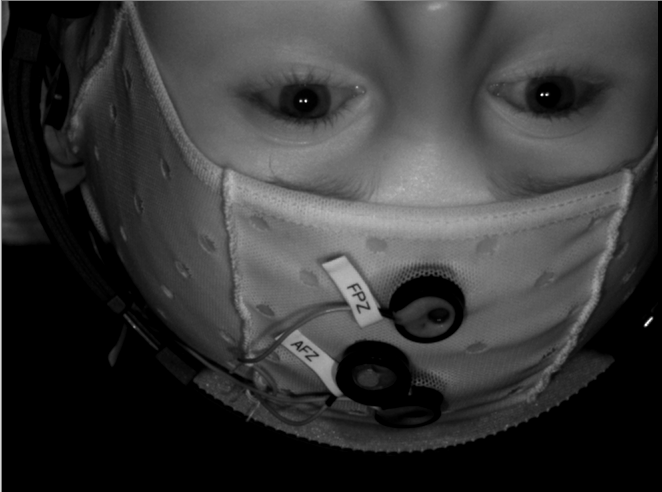
\includegraphics[width=0.7\linewidth]{Billeder/InitialImage.png}
	\caption{Enkelt billede fra video optagelse}
	\label{fig:InitialImage}
	\end{figure}
	
	
	
	Bemærk at procestiden er opgivet som procentdel af samlet procestid, og at værdierne kun omfatter processen selv, og ikke medregner den tid der bruges på metoder der kaldes undervejs. Procestiden for disse metodekald står ud for de enkelte metoder i stedet.
	
	\subsection{Algoritme Oversigt}
	\begin{figure}[h]
		\centering
		\includegraphics[width=0.7\linewidth]{../Algoritmediagram.png}
		\caption[Systemdiagram]{Systemdiagram for Real-time eye-tracking}
		\label{fig:Systemdiagram}
	\end{figure}
	
	\subsubsection{Calculate pupil and gaze}
	
	Main funktion - 0.17%
	
	\subsubsection{Locate corneal reflection}
	
	Finder reflektionspunker - 0.3%
	
	\subsubsection{Starburst pupil contour detection}
	
	Starburst algoritme - 0.63%
	
	\subsubsection{Locate Edge Points}
	
	Find pupil kant punkter - 44.71%
	
	\subsubsection{Fit ellipse ransac}
	
	Tilpas en ellipse til punkterne - 11.7%
	
	\subsection{Fokuspunkter}
	I det følgende underafsnit vil der kort blive beskrevet hvilke dele af systemet der med fordel kan fokuseres på. Dette er baseret på antal gange rutinen bliver kørt, samt hvor lang tid det tager for processen at blive færdig. Begrundelsen for dette er at det højst sandsynligt er lettere at øge performance med en betydelig del hvis de dele der tager længst tid først bliver optimeret.
	
	\subsubsection{Kantdetektion}
	Den mest tidskrævende del af algoritmen er selve starburst-delen, altså den del hvor pupilkantpunkter findes. Udover at optimere koden ved at køre i C, er der også mulighed for at justere variabler for at få processen til at tage kortere tid. Dette vil dog højst sandsynligt ske på bekostning af resultaternes nøjagtighed/præcision, eller systemets overordnede stabilitet. Der vil altså formentligt være behov for en balancering af performance overfor kvalitet. Denne balancering vil foregå iterativt i løbet af implementeringsfasen af projektet.
	
	\subsubsection{Ellipse Tilpasning}
	Den næstmest tidskrævende del af algoritmen er ellipsetilpasningen. Her vil det igen være muligt at justere på variabler, for at balancere performance og kvalitet. Derudover skal der ses nærmere på undtagelsestilstande hvor algoritmen gentages mange gange, RANSAC iterations = 10000. Hvis disse undtagelsestilstande opsluger meget tid og sker ofte, kunne det have en markant effekt på performance for systemet.
	
	\subsubsection{Kegleparametre til Ellipseparametre}
	En mindre betydelig, men dog stadig mærkbar del af algoritmen er den del som oversætter kegleparametre til ellipseparametre. Da denne del af algoritmen kun udgør omkring 6 procent af den samlede procestid, er denne blot nævnt som en mulig kandidat for optimering hvis de primære dele begynder at være sammenlignelige i procestid. 
	
	\subsubsection{Kamera Input}
	En sidste ting der med fordel kan fokuseres på at forbedre er indlæsning af data fra kameraet. Idet der ikke sker meget kompression bør det meste af arbejdet bestå af overførsler i harddisken, men hvis det viser sig at være for tungt kan vi forsøge at gøre noget.
	\subsection{OpenEyes og Siboska}
	Tidligt i projektforløbet blev der udleveret kildekode til gruppen, kildekode som prototypen overvejende er inspireret af "Siboskas kode". Derudover er der også kildekoden som Siboska implementeringen har taget sit
	udspring i. Væsentlige forskelle og egenskaber vil kort blive gennemgået, og en mere grundig gennemgang kan findes i analysedelen af dokumentationen "Ref".
	
	 hvilket også indebærer processeringstid for de enkelte subrutiner. I forlængelse af dette vil begrundelserne for krav der har med algoritmen at gøre også blive givet i en relevant kontekst.
	I det følgende vil simuleringer i forbindelse med starburst algoritmen blive gennemgået. Disse simuleringer er blevet udført i et forsøg på at danne en bedre indsigt i sammenhængen imellem performance og resultater. Idet en overgang til en anden platform end MATlab formentligt ikke forøger performance tilstrækkeligt, skal der i stedet undersøges hvorvidt det er muligt at tilpasse forskellige variabler til at opnå en kortere processeringstid, alt imens resultaterne forbliver gode.
	
	\subsection{Simulering}
	
	Simuleringerne er foretaget med det kode og videodata som Daniel Sibozka har udleveret til gruppen. I det første afsnit vises resultaterne, og i andet afsnit beskrives hvilke ændringer af variabler der afprøves, og derefter vises resultaterne af disse ændringer.
	
	\subsubsection{Extract gaze vector from video}
	
	Processeringstid, CPU = 2.4 GHz
	
	Figur over resultater.
	
	\subsubsection{Variabel Ændringer}
	
	Antal Rays
	Antal RANSAC iterationer
	
	
	\subsubsection{Resultater}
	
	Figur 
	\subsection{Diskussion}
		
\end{document}
\documentclass[rapport.tex]{subfiles}

\begin{document}
	\section{Design}
	For at oprette en software arkitektur der overholder de krav stillet i kravspecifikationen, er der gjort brug af UML (Unified Modelling Language) \cite{UML}. UML tillader en tilnærmelsesvis direkte omskrivning af krav opstillet som use cases, til UML-diagrammer der skitserer en software arkitektur. 
	Da der i kravspecifikationen er gjort brug af UML til udarbejdelse af de forskellige use cases, har det derfor været muligt af skrive sekvensdiagrammer ud fra hver enkelte use case. 
	
	Sideløbende med udviklingen af sekvensdiagrammerne er de forskellige klasser blevet forfattet. Følgende afsnit beskriver grundlæggende tanker og argumentation for valget af klasser.
	\subsection{Indledning}
	Kort om hvad dette afsnit indeholder, og hvorfor det er relevant. 	
	\subsection{Modularisering}
	Programmet er ønsket opbygget, så der af en udestående person, er mulighed for fremtidig ændringer i algoritmen. Programmet er derfor struktureret op omkring at have et fastlagt interface med konsistente input/outputs med en selvstændig algoritme-klasse. 
	\subsection{Applikationsarkitektur}
	Forklaring af overgangen fra use case til software arkitektur. Eksempel med uc3
	
	\begin{figure}
		\centering
		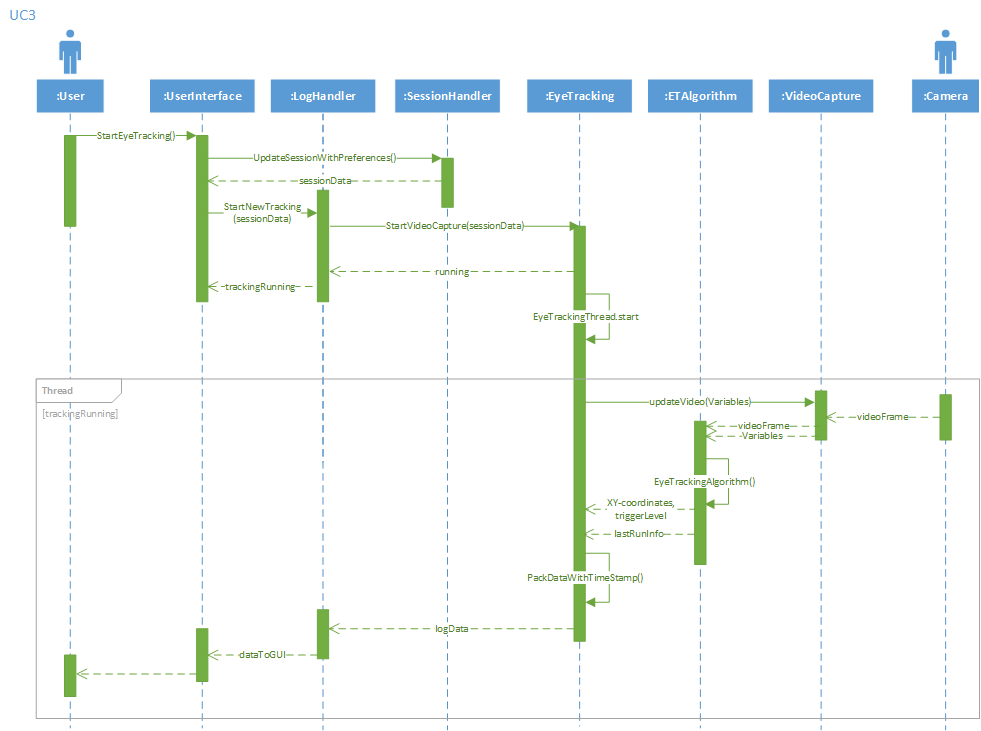
\includegraphics[width=1\linewidth]{UC3}
		\caption[Sekvensdiagram - UC3]{Sekvensdiagram for use case 3 - Start måling}
		\label{fig:UC3}
	\end{figure}
	
	Overvejelser om opdelingen af klasser. Hver klasse varetager en opgave med henblik på en af systemets grænseflader. GUI er varetaget af en klasse. De tre genererede filer log, session, og kalibrering er håndteret af tre klasser. Kommunikation med eksternt kamera er håndteret af sin egen klasse. Kommunikation med algoritmen har sin egen klasse. 
		\subsubsection{UserInterface}
		Denne klasse foretager al kommunikation med aktøren \textit{bruger} igennem et grafisk bruger-interface (GUI). For at have en konstant opdatering af interfacet, forventes denne klasse at blive afviklet i egen tråd. 
		\subsubsection{SessionHandler}
		Her håndteres al data tilknyttet opsætning af eye-tracking-session. 
		\subsubsection{LogHandler}
		Denne klasse håndterer eye-tracking-programmets log-fil. Data fra eye-tracking bliver her pakket og gemt i en log-fil. Kommunikation af målings-relevant data til UserInterface-klassen foretages af denne klasse.
		\subsubsection{VideoCapture}
		\subsubsection{EyeTrackingHandler}
	 
		
		\subsubsection{Interaktion mellem klasser}
		
		\begin{figure}
		\centering
		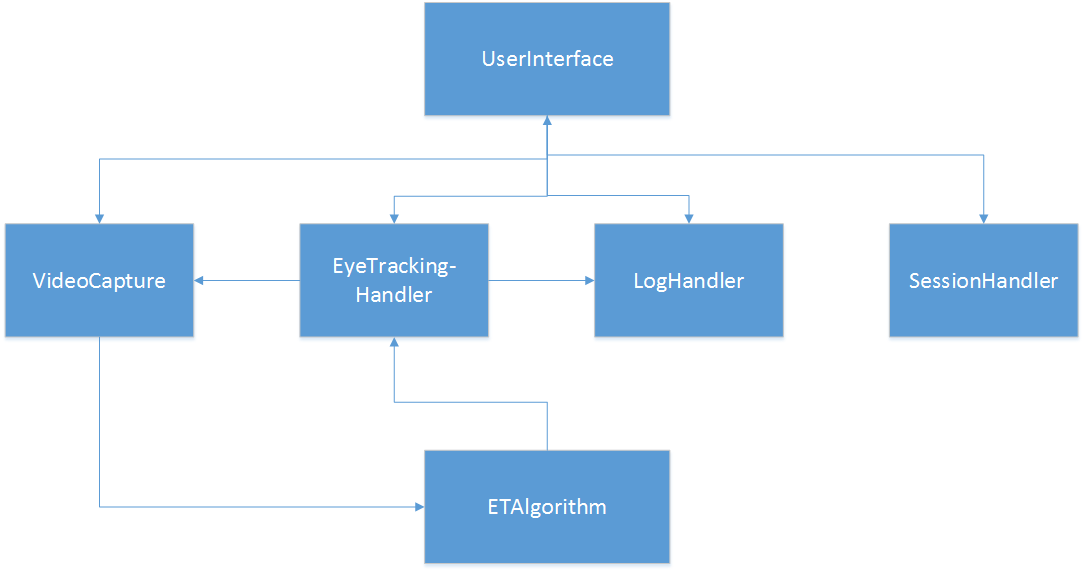
\includegraphics[width=0.8\linewidth]{klasseinteraktion}
		\caption{}
		\label{fig:klasseinteraktion}
		\end{figure}
	\subsection{Algoritme-arkitektur}
	Klassen ETAlgorithm er kernen af eye-tracking-systemet. Her foretages alle udregninger med henblik på eye-tracking. Denne klasse ønskes isoleret så meget som muligt fra resten af systemet, således at der altid kan foretages ændringer i klassens interne kode, uden at det påvirker resten af systemet. Konsistente grænseflader for denne klasse er derfor essentielt. 
	ETAlgorithm bliver håndteret af klassen EyeTracking, modtager et videosignal og et sæt af variabler, og returnerer XY-koordinat, trigger-niveau, samt et sæt af variabler. 
	
	Da program API'en skal kunne understøtte forskellige typer af eye-tracking-algoritmer, har det været nødvendigt at definere inputs og outputs for algoritmeklasse ETAlgorithm. Input-strukturen består af en video-frame i korrekt format givet af OpenCV-arkitekturen, kalibreringsdata, og et sæt af 16 frie variabler. Disse variabler har på forhånd ikke noget format, og giver derfor brugeren mulighed for at videregive en række værdier til algoritmen uanset format. Herved kan enhver algoritme med op til 10 inputvariabler implementeres uden nødvendighed for ændringer i API'en.\\
	\\
	 For eksempel benytter dette projekt sig af en række variabler til at angive: koordinater for sidste pupil-center, afgrænsninger af sidste sæt øjne, hvorvidt Viola Jones skal køres, thresholdværdier, og maks antal RANSAC-iterationer.  Disse værdier indeholder både arrays, matricer, enkelt værdier og  booleans.
	\\
	De 16 frie inputvariablers startværdier kan indstilles fra GUI, og gemmes i præference-filen. 
	\subsection{Bruger-interface}
	Interfacet er designet med henblik på intuitivt brug, så ledes at det ikke er nødvendigt med dybere introduktion til programmet. Forskellige stadier af hvad man kan gøre i interfacet reducerer muligheden for uønskede handlinger. Det er for eksempel ikke muligt at starte eye-tracking før nødvendig opsætning er fuldført. 
	
	Følgende figurer beskriver det forventede grafiske bruger interface. Interfaces er designet ud fra use case diagrammerne beskrevet i kravspecifikationen.
	\subsection{Diskussion}
\end{document}
\documentclass[rapport.tex]{subfiles}

\begin{document}
\section{Implementering}
	\subsection{Indledning}
	\subsection{Bruger-interface og applikation}
	I følgende afsnit vil implementeringen af bruger-interfacet og applikationen blive beskrevet. 
	

	\subsubsection{UserInterface}

	\begin{figure}
	\centering
	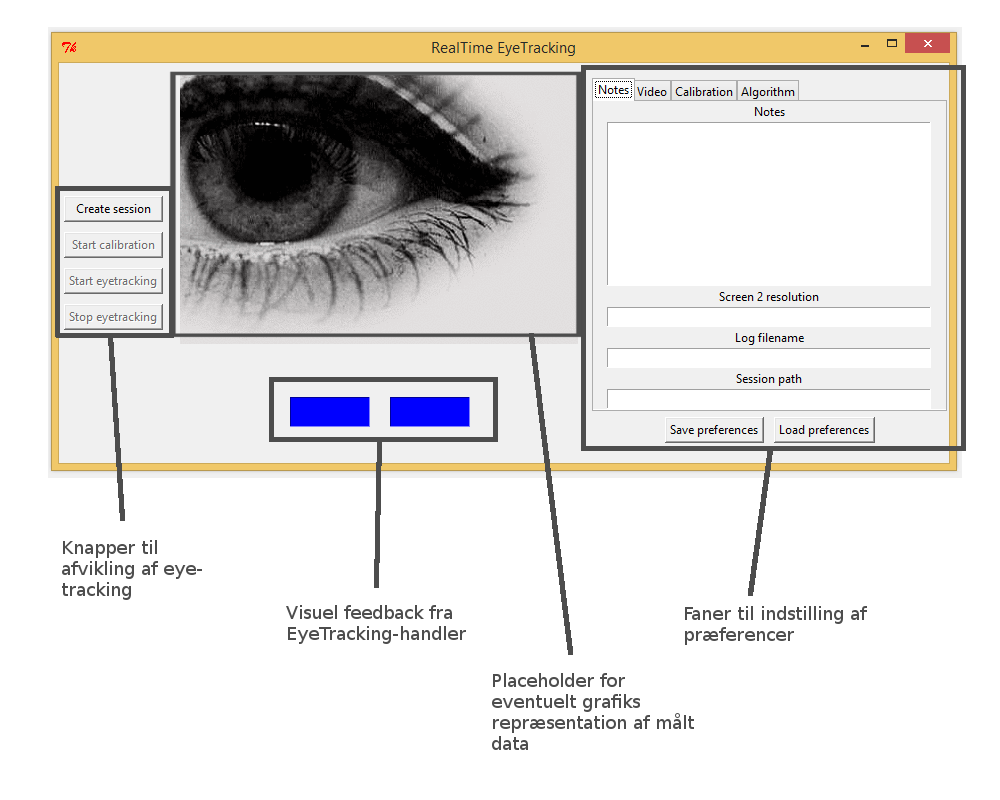
\includegraphics[width=0.9\linewidth]{GUIkommentare}
	\caption[Implementering af GUI]{Implementeringen af det grafiske user-interface med kommentarer}
	\label{fig:GUIkommentare}
	\end{figure}
	
	Tkinter objekter (se afsnit \ref{sec:relBib}) er benyttet til at opbygge det grafisk brugerinterface som givet i design. 
	Hver knap er blevet oprettet med et tilknyttet funktionskald der udfører den ønskede funktion, som givet af de forskellige use cases. 
	Brugeren ser kun Tkinter objekter. 
	Knapperne til venstre i interfacet er sat i rækkefølge efter naturlig opsætning og eksekvering af real-time eye-tracking. Ikke tilgængelige funktioner har deaktiverede knapper således at man ikke kan foretage ulovlige handlinger. \\
	
	De fire faner til højre er til indstilling af præferencer. Herfra kan man tilgå, læse og ændre alle præferencer, samt gemme og indlæse præference-filer.\\
	
	I bunden af bruger-interfacet er to farvede bokse. Disse bokse bruges til at give visuelt feedback bestemt af klassen EyeTrackingHandler. Farven blå indikerer at der ikke kører nogen eye-tracking. Grøn indikerer at eye-tracking kører. Igennem EyeTrackingHandler er det muligt at sætte farven på de to bokse til rød, hvilket kan bruges til at indikere eventuelle fejl. I denne implementering med Starburst-algoritmen er hver boks sat til at repræsentere et øje, således at rød farve indikerer at algoritmen ikke kan finde det tilsvarende øje. 
	Interaktion med andre klasser:
	For hver tilgang til præference-filen bliver der oprettet en ny instans af dataklassen SessionData fra klassen SessionHandler. Ved at aflæse indholdet/værdien af de forskellige Tkiner-objekter og skrive dette data til den instansen af SessionData, der senere bliver skrevet til præference-filen af klassen SessionHandler, vil der altid være konsistens mellem værdierne skrevet i brugerinterfacet, værdierne i præference-filen, og værdierne brugt i eye-tracking-algoritmen. 
	
	Programbibliotekerne tkFileDialog og tkMessageBox giver værktøjer til at kommunikere med brugeren. tkFileDialog håndterer arbejdet med valg af filer, og giver brugeren mulighed for at bevæge sig rundt i mapper på computeren. tkMessageBox bruges til pop-up-vinduer, hvilket benyttes til at tvinge brugeren til at gennemføre valg for at fortsætte, samt til at prompte brugeren om fejl og ulovlige handlinger. 
	
	
	\subsubsection{SessionHandler}
	SessionHandlers opgave er at stille et data-format til rådighed for kommunikation af sessions-indstillinger de forskellige klasser imellem. Klassens vigtigste opgave er derfor at opretholde et korrekt format. Ved oprettelse eller opdatering af præference-fil, kreerer SessionHandler en streng med henholdsvis navn på variabeltype, variable værdi konverteret til streng (hvis variablen er tom, skrives strengen "None"), efterfulgt af et linebreak. Når strengen er oprettet for alle variabler, skrives strengen til en præference-fil med suffiks .pref. \\
	Når en præference-fil indlæses, verificeres den først af SessionHandler ved at lede efter alle variablenavne i den læste fil. Herefter kan hver variabel udtrækkes fra filen. Det er nødvendigt at lave tjek på hver variabel, da konvertering fra python- og numpy-værdi til streng kan medføre komplikationer. 
	
	Instanser af SessionHandler brugt som data-format bliver oftest omtalt som SessionData.\\
	
	Figur \ref{list:sessionfile} er et eksempel på præference-fil med korrekt format (Værdierne variablenames og variablevalues er trunkeret for formateringens skyld). 
\begin{figure}
\caption{Eksempel på præference-fil}
\label{list:sessionfile}
\begin{lstlisting}
SESSIONPATH C:/RealTimeEyeTracking
USINGCAM True
CAMNR None
VIDEOPATH 0
NOTES Dette er en testsession
RESOLUTION 1600x900
CALTYPE Numbers
LOGFILENAME testlog
CALFILENAME testcallog
LOADEDCALDATA None
RECORDVIDEO False
RAWDATAPATH None
VARIABLENAMES['e_center', 'last_eyes', ...
VARIABLEVALUES['[0,0]'$  '[]'$ 'True'$ '20'$ '1500'$ ...
\end{lstlisting}
\end{figure}
		
	\subsubsection{LogHandler}
	For hver eye-tracking måling der igangsættes bliver der oprettet en instans af LogHandler klassen med argumentet SessionData, som er en instans af klassen SessionHandler. LogHandler-klassen består af tre simple funktioner: StartNewTracking, StopTracking og LogData. StartNewTracking er en del af kommunikationsvejen fra UserInterface til EyeTrackingHandler, og har til formål at pege på sig selv, således at EyeTrackingHandler kan kalde LogData i den rette instans af klassen. 
	Ligeledes StartNewTracking er StopTracking en del af kommunikationsvejen, men har kun til formål at sætte klassens variabel Tracking til False. Funktionen LogData bliver kaldt fra EyeTrackingHandler med en streng som argument, og har til formål at skrive denne streng - efterfulgt af et linebreak - til en log-fil peget på af SessionData.  
	
	Figur \ref{list:logfile} er et eksempel på en log-fil med korrekt format (Timestamp, X, Y, Triggerniveau, Fejlmeddelelse). 
\begin{figure}
	\caption{Eksempel på log-fil}
	\label{list:logfile}
	\begin{lstlisting}	
16:28:46.483000, 89, 69, 0, None
16:28:46.662000, 89, 69, 0, None
16:28:46.731000, 90, 70, 0, None
16:28:46.782000, 90, 71, 0, None
16:28:46.951000, 92, 74, 0, None
16:28:47.093000, 89, 68, 0, None
16:28:47.244000, 89, 51, 1, None
16:28:47.322000, 89, 52, 1, None
16:28:47.360000, 91, 52, 1, None
16:28:47.395000, 89, 51, 1, None
16:28:47.598000, 0, 0, 0, Maximum ransac iterations exceeded
16:28:47.651000, 89, 51, 1, None
\end{lstlisting}
\end{figure}	
	
	\subsubsection{CalibrationHandler}
	Vis eksempel på kalibrerings-fil
	
	\subsubsection{EyeTrackingHandler}
	
	
	\subsubsection{VideoCapture}
	Indeholder puplic funktion GetCameraInputs. 
	Andre funktioner er en del af klassen. Klassen oprettes med et video-input, og mulighed for kalibreringsdataet, samt ti frie variabler. Kalibreringsdataet og de ti frie variabler benyttes ikke til andet end at videresende til ETAlgorithm sammen med gyldig frame. 
	At passe kalibreringsdataet og de frie variabler igennem VideoCapture er ikke optimalt, men spiller ingen rolle i det samlede arbejdslæs. Det kan forestilles at man i stedet ville sende to pointers til hvor disse data ville være lageret. Argumentet for at passe disse data igennem VideoCapture er, at VideoCapture så vil kalde ETAlgorithm's Track() med den fundne frame samt disse data, i stedet for at returnere den fundne frame til EyeTrackingHandler og derefter kalde Track(). VideoCapture håndterer al kommunikation med video-kameraer, og har tilsvarende ansvaret for at terminere forbindelsen med disse når en måling er overstået. 
		
	\subsubsection{Kommunikation imellem applikationens klasser}	
	
	Overordnet kan programmet befinde sig i tre stadier: NotRunning, Calibrating og Running. 	
	
	\subsection{ETAlgorithm}
	Koden i figur \ref{list:emptyalg} er en tom udgave af klassen ETAlgorithm med de nødvendige input-argumenter og funktionskald til EyeTrackingHandler er implementeret:

\begin{figure}
	\caption{Tom udgave af klassen ETAlgorithm}
	\label{list:emptyalg}
\begin{lstlisting}
import numpy as np
import EyeTracking as et

#Her tilfoejes diverse python-biblioteker

def Track(frame, calibration_data, variables):

#Egen kode her 

et.PackWithTimestamp(screen_point, trigger_value)
et.LastRunInfo(variables)
return
\end{lstlisting}
\end{figure}

	
	
	Afsnit \ref{StarburstImpl} beskriver implementering af Starburst-algoritmen i ETAlgorithm.
	\subsection{Starburst-algoritmen}
	\label{StarburstImpl}
	\subsection{Optimering}
	
	\subsubsection{Fremtidige optimeringsmuligheder}
	Python understøtter multitrådning, hvilket giver mulighed for at køre flere instanser af eye-tracking-algoritmen sideløbende. Skriv mere om muligheder for multitrådning, og hvorfor det kan virke.
	\subsection{Diskussion}
		
\end{document}
\documentclass[rapport.tex]{subfiles}

\begin{document}
\section{Test}
	\subsection{Indledning}
	\subsection{Deltest}
	Deltestene har til formål at teste hver enkelte klasses funktionalitet. 
	Da de forskellige klasser er skrevet i hver sin python-fil, og da python-filer uden problemer kan inkluderes i python-programmer, har hver klasse været mulig at teste ved at skrive kalde funktionaliteter med specifikke inputs og derefter læse returværdierne/observere hændelserne. \\
	
	Ved at skrive en test-bench (her et python-program) har det været muligt at teste hver klasses funktionaliteter. Alle test-cases er udført i værktøjet Visual Studio, hvilket giver fri mulighed for at aflæse de forskellige variabler i runtime. Følgende er kort beskrivelse af deltest og resultater for hver klasse:
	\begin{itemize}
		\item \textbf{UserInterface}: Klassen er testet ved at køre programmet og observere at: Bruger-interfacet indeholder de samme knapper og tekstfelter som angivet i softwarearkitekturen, knapperne forsøger at kalde de rigtige funktioner når der trykkes på dem, man kan aflæse korrekte værdier i tekstfelterne, og at både program og bruger kan skrive værdier i tekstfelterne. 
		\item \textbf{SessionHandler}: Her er testet at en oprettet instans af klassen kan: Gemme egen data i en fil, læse og sætte egen data fra en fil, og verificere korrekt - eller afvise ugyldigt - filformat.
		\item \textbf{LogHandler}: Her er testet at en oprettet instans af klassen kan: Oprette log-fil ud fra givet filsti og navn og tilføje strenge med korrekt format til den angivne log-fil.
		\item \textbf{EyeTrackingHandler}: Denne klasse er først testet for de funktionskald der skal komme fra ETAlgorithm. Her er testet at den kan: Modtage resultater og tilføje et korrekt timestamp til dem, modtage en fejlmeddelelse og tilføje et korrekt timestamp, formatere en streng i outputformatet givet i kravspecifikationen, og modtage et array på ti variabler. Herefter er det testet at klassen kan oprette en process hvori en tråd gentager sig selv med en hastighed på 1/opdateringshastighed sekunder.
		\item \textbf{VideoCapture}: Her er der testet at klassen kan benytte OpenCV til at detektere og benytte video-hardware, læse videofiler, samt læse opdateringshastigheden fra video-hardware og videofiler, eller sætte en standard hastighed hvis ingen kunne læses (noget video-hardware kan ikke aflæses). \\
	\end{itemize}
	Hvis nogle punkter ikke har kunne godkendes når denne test har været kørt, har det været muligt at gå tilbage og ændre i implementeringen.
	\subsection{Integrationstest}
	Integrationstesten har til formål at teste kommunikationen klasser imellem.  Ligesom i deltesten har denne test kunne udføres ved hjælp af en test-bench, dog med to klasser benyttet af gangen. Hver kommunikationsvej (som set på figur \ref{fig:klasseinteraktion}) er her testet. Funktionskald og de dertilhørende argumenter er i denne test blevet verificeret. 
	Denne test har ikke medført nogle problemer, da der i softwarearkitekturen har været defineret en klar kommunikation klasserne imellem, og da Python benytter sig af et høj-niveau data-typer.
	
	\subsection{Accepttest}
	Accepttesten er formuleret efter de opstillede krav i afsnit \ref{sec:kravspec}. Formålet ved accepttesten er at teste det samlede produkt op imod de stillede krav. Testen afsluttes når alle specificerede test cases er gennemført og godkendt. I tilfælde hvor et krav ikke har kunne fuldføres, er der udfærdiget en problemrapport årsagen til underkendelsen. 
	
	\subsection{Performance-evaluering}
	\subsection{Diskussion af testresultater}
		
\end{document}
\documentclass[rapport.tex]{subfiles}

\begin{document}
\section{Konklusion}
	
		
\end{document}
\documentclass[rapport.tex]{subfiles}

\begin{document}
\section{Appendiks}	
På vedlagt CD findes alle billag navngivet som følgende:
	\begin{itemize}
		\item A - Rapport.pdf
		\item B - Kravspecifikation.pdf
		\item C - Analyse.pdf
		\item D - Softwarearkitektur.pdf
		\item E - Programkode.zip
		\item F - Accepttest.pdf

	\end{itemize}

		
\end{document}
\printbibliography

\end{document}